\section{Cruscotto di valutazione della qualità}
\subsection{MPC01-EAC (Estimated at Completition)}
Dal grafico si può notare che l'EAC supera il valore accettabile di quest'ultimo. La causa di questa situazione si può ricondurre principalmente alla quasi assente divisione delle ore individuali e le ore produttive.
\subsection{MPC02-PV (Planned Value) e MPC04-EV (Earned Value)}
Dal grafico si può notare che le linee del PV e dell'EV sono molto vicine fra loro, ciò implica che il lavoro svolto è conforme a quello pianificato.
\subsection{MPC05-ETC (Estimated to Complete)}
Dal grafico si può notare che le linee dell'AC e dell'ETC nel corso dei vari periodi, mantengano un andamento costante. Di conseguenza si può affermare che il progetto stia mantenendo un ritmo regolare di avanzamento. 
\subsection{MPC08-BV (Budget Variance)}

\subsection{MPC09-RSI (Requirements stability index)}
\subsection{MPC14-IG (Indice Gulpeanse)}
\subsection{MPC15-NCR (Non Calculated Risk)}
\begin{figure}[H]
  \centering
  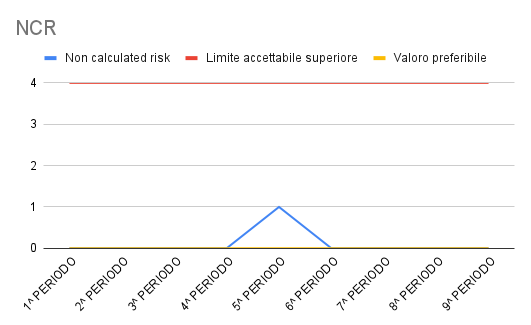
\includegraphics[width=0.7\linewidth]{grafici/NCR.png}
  \caption{Non Calculated Risk}
\end{figure}
Dal grafico si può notare che per la maggior parte del tempo non sono comparsi rischi non previsti. Solo nel quinto periodo si è emerso un rischio di cui non si era tenuto conto inizialmente, ovvero la sessione di esami, la quale ha portato via parecchio tempo ai vari membri del gruppo, rallentando di molto l'avanzamento del lavoro.
\subsection{MPC16-ET (Efficienza temporale)}
